\documentclass[11pt]{article}

\usepackage{graphicx} % gere les images 
\usepackage[utf8]{inputenc} % pour les accents
\usepackage{hyperref}
\usepackage[french]{babel}

\begin{document}

\begin{titlepage}
	\newcommand{\HRule}{\rule{\linewidth}{0.2mm}}     
            
	\begin{figure}[t]
		\begin{minipage}{0.5\textwidth}\large
			\begin{flushleft}
				
\includegraphics[width=0.7\textwidth]{assets/logoEsirem.jpg}
			\end{flushleft}
		\end{minipage}
		\begin{minipage}{0.5\textwidth}\large
			\begin{flushright}
			
\includegraphics[width=0.6\textwidth]{assets/logoUb.jpg}
			\end{flushright}
		\end{minipage}
	\end{figure}
	\textsc{ \\[1cm]}
     
     
	\begin{center}
	\HRule \\
	{\Large   
		Mettre titre
	}
	\HRule
	\\[0.5cm]
	{\large Rapport réseau \\}
   \end{center}

	\begin{figure}[h]
		\begin{center}
			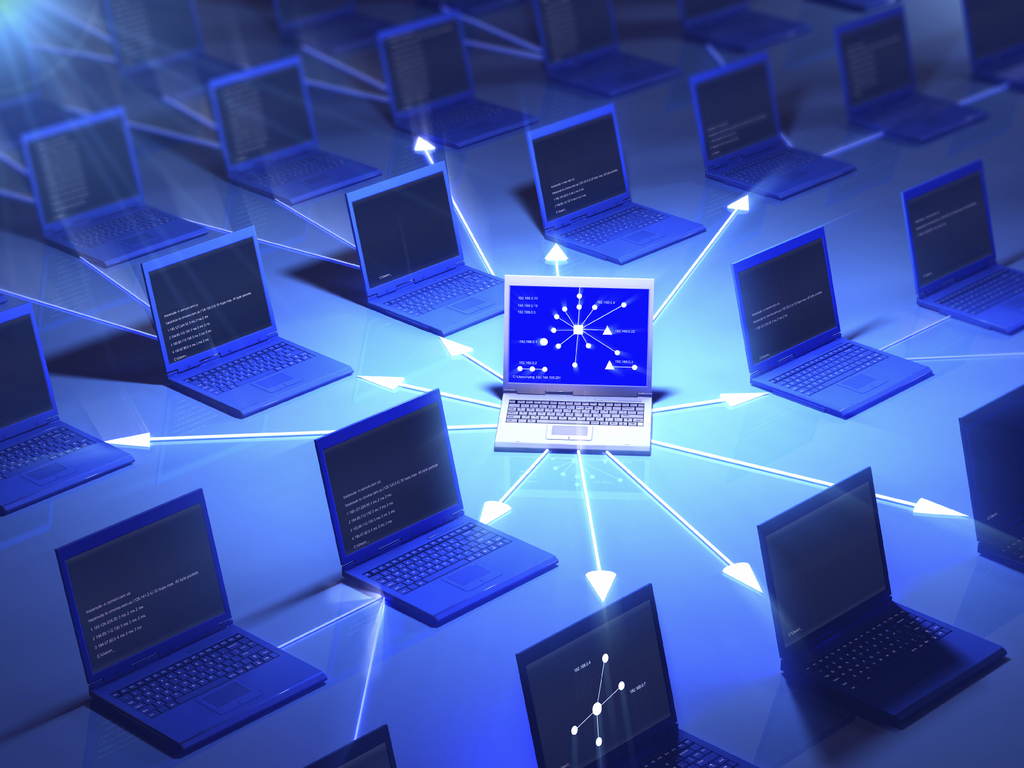
\includegraphics[width=0.4\textwidth]{assets/main.jpg}
		\end{center}
	\end{figure}
        
	\vfill 
	\begin{center}
        \textsc{\large
        	ESIREM \\
			École Supérieure d'Ingénieurs de Recherche en Matériaux et en Infotronique\\       	
			[2cm]
		}
	\end{center}

	\begin{minipage}{0.5\textwidth}
		\begin{flushleft} \large
			\emph{Auteurs:}\\
			Armen Mahmedov \\
			Aurélien Patru
		\end{flushleft}
	\end{minipage}
	~
	\begin{minipage}{0.5\textwidth}
		\begin{flushright}\large
			\emph{Professeur :} \\
			Nader Mbarek \\
		\end{flushright}
	\end{minipage}
        
\end{titlepage}
  
% saut de page  ou   ~ \pagebreak 
\newpage
\strut
\newpage

\tableofcontents


\pagebreak

Introduction générale 


\section{Découvert de NS-2 et nam}
[introduction de la partie]

\subsection{Sous-partie 1}


[conclusion de la partie]

\section{TP 2}
\subsection{Sous-partie 1}


\section{TP 3}
\subsection{Sous-partie 1}




















\end{document}
